\documentclass{article}\usepackage[]{graphicx}\usepackage[]{xcolor}
% maxwidth is the original width if it is less than linewidth
% otherwise use linewidth (to make sure the graphics do not exceed the margin)
\makeatletter
\def\maxwidth{ %
  \ifdim\Gin@nat@width>\linewidth
    \linewidth
  \else
    \Gin@nat@width
  \fi
}
\makeatother

\definecolor{fgcolor}{rgb}{0.345, 0.345, 0.345}
\newcommand{\hlnum}[1]{\textcolor[rgb]{0.686,0.059,0.569}{#1}}%
\newcommand{\hlsng}[1]{\textcolor[rgb]{0.192,0.494,0.8}{#1}}%
\newcommand{\hlcom}[1]{\textcolor[rgb]{0.678,0.584,0.686}{\textit{#1}}}%
\newcommand{\hlopt}[1]{\textcolor[rgb]{0,0,0}{#1}}%
\newcommand{\hldef}[1]{\textcolor[rgb]{0.345,0.345,0.345}{#1}}%
\newcommand{\hlkwa}[1]{\textcolor[rgb]{0.161,0.373,0.58}{\textbf{#1}}}%
\newcommand{\hlkwb}[1]{\textcolor[rgb]{0.69,0.353,0.396}{#1}}%
\newcommand{\hlkwc}[1]{\textcolor[rgb]{0.333,0.667,0.333}{#1}}%
\newcommand{\hlkwd}[1]{\textcolor[rgb]{0.737,0.353,0.396}{\textbf{#1}}}%
\let\hlipl\hlkwb

\usepackage{framed}
\makeatletter
\newenvironment{kframe}{%
 \def\at@end@of@kframe{}%
 \ifinner\ifhmode%
  \def\at@end@of@kframe{\end{minipage}}%
  \begin{minipage}{\columnwidth}%
 \fi\fi%
 \def\FrameCommand##1{\hskip\@totalleftmargin \hskip-\fboxsep
 \colorbox{shadecolor}{##1}\hskip-\fboxsep
     % There is no \\@totalrightmargin, so:
     \hskip-\linewidth \hskip-\@totalleftmargin \hskip\columnwidth}%
 \MakeFramed {\advance\hsize-\width
   \@totalleftmargin\z@ \linewidth\hsize
   \@setminipage}}%
 {\par\unskip\endMakeFramed%
 \at@end@of@kframe}
\makeatother

\definecolor{shadecolor}{rgb}{.97, .97, .97}
\definecolor{messagecolor}{rgb}{0, 0, 0}
\definecolor{warningcolor}{rgb}{1, 0, 1}
\definecolor{errorcolor}{rgb}{1, 0, 0}
\newenvironment{knitrout}{}{} % an empty environment to be redefined in TeX

\usepackage{alltt}
\IfFileExists{upquote.sty}{\usepackage{upquote}}{}
\begin{document}

\section{Question 1}
\begin{knitrout}
\definecolor{shadecolor}{rgb}{0.969, 0.969, 0.969}\color{fgcolor}\begin{kframe}
\begin{alltt}
\hldef{data} \hlkwb{<-} \hlkwd{c}\hldef{(}\hlnum{45}\hldef{,} \hlnum{50}\hldef{,} \hlnum{55}\hldef{,} \hlnum{60}\hldef{,} \hlnum{65}\hldef{,} \hlnum{70}\hldef{,} \hlnum{75}\hldef{,} \hlnum{80}\hldef{)}
\hldef{mean_data} \hlkwb{<-} \hlkwd{mean}\hldef{(data)}
\hldef{median_data} \hlkwb{<-} \hlkwd{median}\hldef{(data)}
\hldef{variance_data} \hlkwb{<-} \hlkwd{var}\hldef{(data)}
\hldef{std_data} \hlkwb{<-} \hlkwd{sd}\hldef{(data)}

\hldef{mean_data}
\end{alltt}
\begin{verbatim}
## [1] 62.5
\end{verbatim}
\begin{alltt}
\hldef{median_data}
\end{alltt}
\begin{verbatim}
## [1] 62.5
\end{verbatim}
\begin{alltt}
\hldef{variance_data}
\end{alltt}
\begin{verbatim}
## [1] 150
\end{verbatim}
\begin{alltt}
\hldef{std_data}
\end{alltt}
\begin{verbatim}
## [1] 12.24745
\end{verbatim}
\end{kframe}
\end{knitrout}
\section{question 2}
\begin{knitrout}
\definecolor{shadecolor}{rgb}{0.969, 0.969, 0.969}\color{fgcolor}\begin{kframe}
\begin{alltt}
\hlkwd{library}\hldef{(datasets)}
\hldef{data} \hlkwb{<-} \hldef{iris}

\hlkwd{boxplot}\hldef{(data}\hlopt{$}\hldef{Sepal.Length)}
\end{alltt}
\end{kframe}
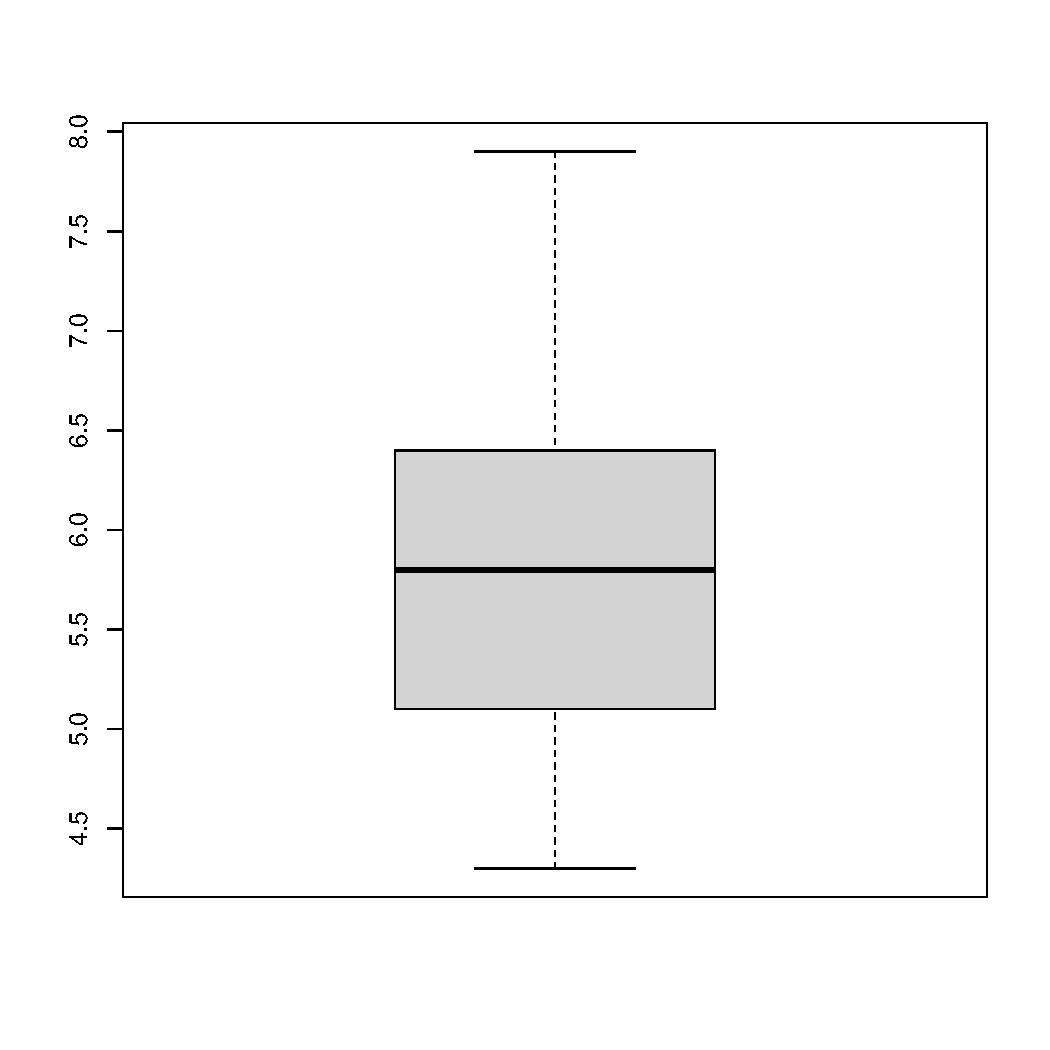
\includegraphics[width=\maxwidth]{figure/unnamed-chunk-2-1} 
\begin{kframe}\begin{alltt}
\hlkwd{plot}\hldef{(data}\hlopt{$}\hldef{Sepal.Length, data}\hlopt{$}\hldef{Petal.Length,} \hlkwc{xlab}\hldef{=}\hlsng{"Sepal Length"}\hldef{,} \hlkwc{ylab}\hldef{=}\hlsng{"Petal Length"}\hldef{)}
\end{alltt}
\end{kframe}
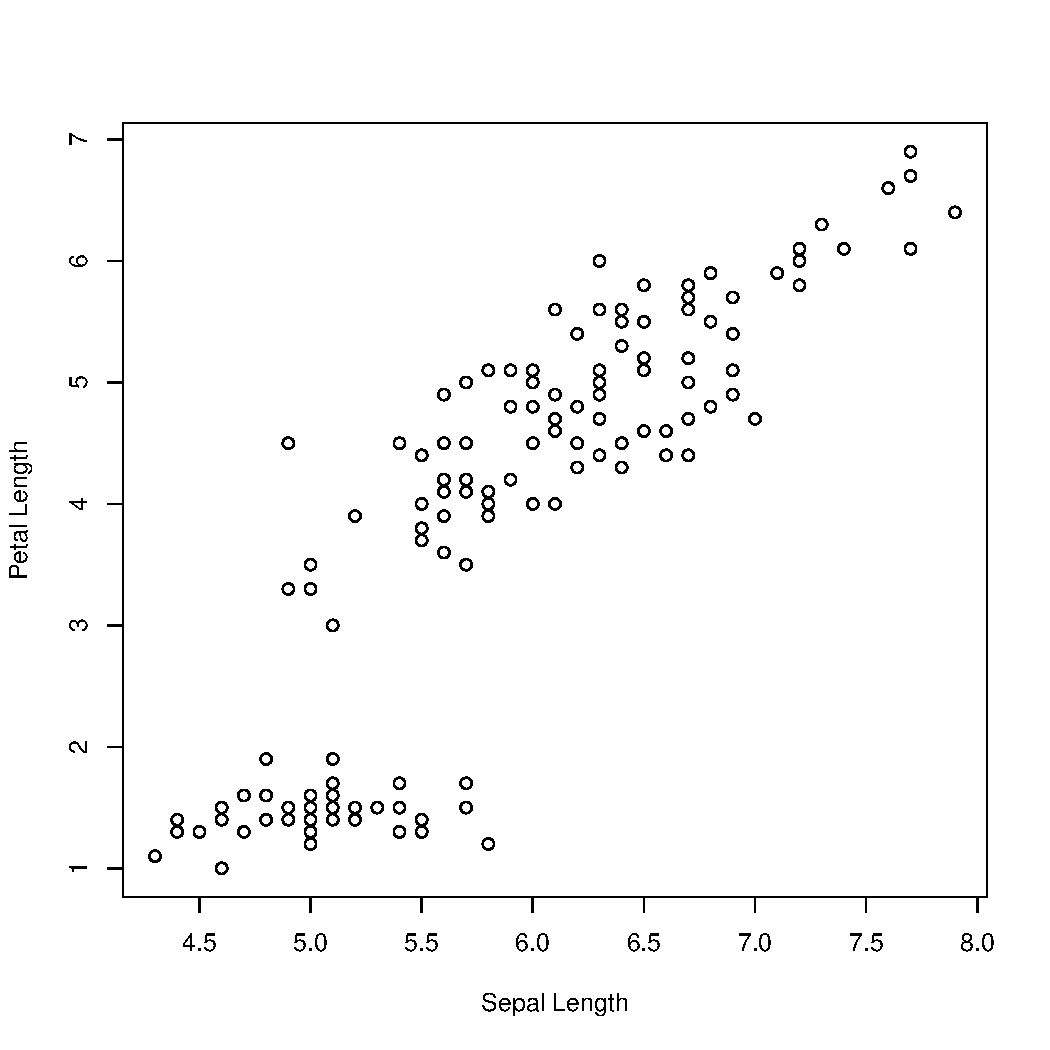
\includegraphics[width=\maxwidth]{figure/unnamed-chunk-2-2} 
\end{knitrout}
\section{question 3}
\begin{knitrout}
\definecolor{shadecolor}{rgb}{0.969, 0.969, 0.969}\color{fgcolor}\begin{kframe}
\begin{alltt}
\hlcom{#Null hypothesis: There is significant differences}
\hlcom{#Alter hypo: There is significant difference.}
\hldef{brand_a} \hlkwb{<-} \hlkwd{c}\hldef{(}\hlnum{12.4}\hldef{,} \hlnum{13.1}\hldef{,} \hlnum{14.2}\hldef{,} \hlnum{15.0}\hldef{,} \hlnum{13.8}\hldef{)}
\hldef{brand_b} \hlkwb{<-} \hlkwd{c}\hldef{(}\hlnum{11.9}\hldef{,} \hlnum{12.5}\hldef{,} \hlnum{13.0}\hldef{,} \hlnum{12.8}\hldef{,} \hlnum{13.2}\hldef{)}

\hldef{t_stat} \hlkwb{<-} \hlkwd{t.test}\hldef{(brand_a, brand_b,} \hlkwc{alternative} \hldef{=} \hlsng{"two.sided"}\hldef{,} \hlkwc{var.equal}\hldef{=}\hlnum{TRUE}\hldef{,} \hlkwc{conf.level} \hldef{=} \hlnum{0.95}\hldef{)}
\hldef{t_stat}
\end{alltt}
\begin{verbatim}
## 
## 	Two Sample t-test
## 
## data:  brand_a and brand_b
## t = 2.0343, df = 8, p-value = 0.07634
## alternative hypothesis: true difference in means is not equal to 0
## 95 percent confidence interval:
##  -0.136226  2.176226
## sample estimates:
## mean of x mean of y 
##     13.70     12.68
\end{verbatim}
\begin{alltt}
\hlcom{# given that p_value is 0.07 which is more than 0.05. We reject the null hypothesis that there is significat differences in mean }
\end{alltt}
\end{kframe}
\end{knitrout}

\section{question 4}
\begin{knitrout}
\definecolor{shadecolor}{rgb}{0.969, 0.969, 0.969}\color{fgcolor}\begin{kframe}
\begin{alltt}
\hldef{before} \hlkwb{<-} \hlkwd{c}\hldef{(}\hlnum{15.2}\hldef{,} \hlnum{14.8}\hldef{,} \hlnum{15.5}\hldef{,} \hlnum{16.0}\hldef{,} \hlnum{15.7}\hldef{)}
\hldef{after} \hlkwb{<-} \hlkwd{c}\hldef{(}\hlnum{14.5}\hldef{,} \hlnum{14.0}\hldef{,} \hlnum{14.8}\hldef{,} \hlnum{15.2}\hldef{,} \hlnum{14.9}\hldef{)}

\hldef{t_stat} \hlkwb{<-} \hlkwd{t.test}\hldef{(before, after,} \hlkwc{paired} \hldef{=} \hlnum{TRUE}\hldef{)}
\hldef{t_stat}
\end{alltt}
\begin{verbatim}
## 
## 	Paired t-test
## 
## data:  before and after
## t = 31.027, df = 4, p-value = 6.43e-06
## alternative hypothesis: true mean difference is not equal to 0
## 95 percent confidence interval:
##  0.6919913 0.8280087
## sample estimates:
## mean difference 
##            0.76
\end{verbatim}
\begin{alltt}
\hlcom{# therefore the means are different.}
\end{alltt}
\end{kframe}
\end{knitrout}
\section{question 5}

\begin{knitrout}
\definecolor{shadecolor}{rgb}{0.969, 0.969, 0.969}\color{fgcolor}\begin{kframe}
\begin{alltt}
\hldef{n1} \hlkwb{<-} \hlnum{500}
\hldef{q} \hlkwb{<-} \hlnum{320}
\hldef{alpha} \hlkwb{<-} \hlnum{0.05}

\hldef{prop_stat} \hlkwb{<-} \hlkwd{prop.test}\hldef{(}\hlnum{320}\hldef{,} \hlnum{500}\hldef{,} \hlkwc{p}\hldef{=}\hlnum{0.5}\hldef{,} \hlkwc{alternative} \hldef{=} \hlsng{"greater"}\hldef{,} \hlkwc{correct}\hldef{=}\hlnum{FALSE}\hldef{)}
\hldef{prop_stat}
\end{alltt}
\begin{verbatim}
## 
## 	1-sample proportions test without continuity correction
## 
## data:  320 out of 500, null probability 0.5
## X-squared = 39.2, df = 1, p-value = 1.913e-10
## alternative hypothesis: true p is greater than 0.5
## 95 percent confidence interval:
##  0.6040248 1.0000000
## sample estimates:
##    p 
## 0.64
\end{verbatim}
\begin{alltt}
\hlcom{# given that the p_value is very very small we accept our null hypothesis that more than half the population prefers online shopping.}
\end{alltt}
\end{kframe}
\end{knitrout}

\section{question 6}
\begin{knitrout}
\definecolor{shadecolor}{rgb}{0.969, 0.969, 0.969}\color{fgcolor}\begin{kframe}
\begin{alltt}
\hldef{before} \hlkwb{<-} \hlkwd{c}\hldef{(}\hlnum{72}\hldef{,} \hlnum{75}\hldef{,} \hlnum{78}\hldef{,} \hlnum{80}\hldef{,} \hlnum{74}\hldef{)}
\hldef{after} \hlkwb{<-} \hlkwd{c}\hldef{(}\hlnum{70}\hldef{,} \hlnum{73}\hldef{,} \hlnum{76}\hldef{,} \hlnum{78}\hldef{,} \hlnum{72}\hldef{)}

\hldef{wil_sta} \hlkwb{<-} \hlkwd{wilcox.test}\hldef{(before, after,} \hlkwc{alternative}\hldef{=}\hlsng{"two.sided"}\hldef{)}
\end{alltt}


{\ttfamily\noindent\color{warningcolor}{\#\# Warning in wilcox.test.default(before, after, alternative = "{}two.sided"{}): cannot compute exact p-value with ties}}\begin{alltt}
\hldef{wil_sta}
\end{alltt}
\begin{verbatim}
## 
## 	Wilcoxon rank sum test with continuity correction
## 
## data:  before and after
## W = 17, p-value = 0.4005
## alternative hypothesis: true location shift is not equal to 0
\end{verbatim}
\begin{alltt}
\hlcom{#there is a significat reduction in weight values.}
\end{alltt}
\end{kframe}
\end{knitrout}

\section{question 7}
\begin{knitrout}
\definecolor{shadecolor}{rgb}{0.969, 0.969, 0.969}\color{fgcolor}\begin{kframe}
\begin{alltt}
\hldef{data} \hlkwb{<-} \hlkwd{matrix}\hldef{(}\hlkwd{c}\hldef{(}\hlnum{10}\hldef{,} \hlnum{15}\hldef{,}\hlnum{20}\hldef{,} \hlnum{20}\hldef{,} \hlnum{25}\hldef{,}\hlnum{30}\hldef{,} \hlnum{30}\hldef{,} \hlnum{35}\hldef{,} \hlnum{40}\hldef{,} \hlnum{40}\hldef{,} \hlnum{25}\hldef{,} \hlnum{35}\hldef{),} \hlkwc{nrow} \hldef{=} \hlnum{3}\hldef{)}
\hldef{data}
\end{alltt}
\begin{verbatim}
##      [,1] [,2] [,3] [,4]
## [1,]   10   20   30   40
## [2,]   15   25   35   25
## [3,]   20   30   40   35
\end{verbatim}
\begin{alltt}
\hldef{chi_stat} \hlkwb{<-} \hlkwd{chisq.test}\hldef{(data)}
\hldef{chi_stat}
\end{alltt}
\begin{verbatim}
## 
## 	Pearson's Chi-squared test
## 
## data:  data
## X-squared = 6.7554, df = 6, p-value = 0.3441
\end{verbatim}
\begin{alltt}
\hlcom{# given that the p-value is higher than 0.05, we reject the null hypothesis that the attributes are independent.}
\end{alltt}
\end{kframe}
\end{knitrout}

\section{question 8}

\begin{knitrout}
\definecolor{shadecolor}{rgb}{0.969, 0.969, 0.969}\color{fgcolor}\begin{kframe}
\begin{alltt}
\hlcom{# not sure how to do this}
\end{alltt}
\end{kframe}
\end{knitrout}

\section{question 9}
\begin{knitrout}
\definecolor{shadecolor}{rgb}{0.969, 0.969, 0.969}\color{fgcolor}\begin{kframe}
\begin{alltt}
\hldef{meanwire} \hlkwb{<-} \hlnum{5}
\hldef{stdwire} \hlkwb{<-} \hlnum{0.2}
\hldef{probab} \hlkwb{<-} \hlkwd{pnorm}\hldef{(}\hlnum{5.3}\hldef{,} \hlkwc{mean}\hldef{=meanwire,} \hlkwc{sd}\hldef{=stdwire)}
\hldef{probab}
\end{alltt}
\begin{verbatim}
## [1] 0.9331928
\end{verbatim}
\begin{alltt}
\hlcom{# probability is 0.933 that randomly selected covering has thickness greater than 5.3mm}
\end{alltt}
\end{kframe}
\end{knitrout}
\section{question 10}

\begin{knitrout}
\definecolor{shadecolor}{rgb}{0.969, 0.969, 0.969}\color{fgcolor}\begin{kframe}
\begin{alltt}
\hlcom{# no idea how to proceed here}
\end{alltt}
\end{kframe}
\end{knitrout}
\section{question 11}
\begin{knitrout}
\definecolor{shadecolor}{rgb}{0.969, 0.969, 0.969}\color{fgcolor}\begin{kframe}
\begin{alltt}
\hlkwd{library}\hldef{(datasets)}
\hldef{data} \hlkwb{<-} \hldef{mtcars}

\hlkwd{summary}\hldef{(data)}
\end{alltt}
\begin{verbatim}
##       mpg             cyl             disp             hp       
##  Min.   :10.40   Min.   :4.000   Min.   : 71.1   Min.   : 52.0  
##  1st Qu.:15.43   1st Qu.:4.000   1st Qu.:120.8   1st Qu.: 96.5  
##  Median :19.20   Median :6.000   Median :196.3   Median :123.0  
##  Mean   :20.09   Mean   :6.188   Mean   :230.7   Mean   :146.7  
##  3rd Qu.:22.80   3rd Qu.:8.000   3rd Qu.:326.0   3rd Qu.:180.0  
##  Max.   :33.90   Max.   :8.000   Max.   :472.0   Max.   :335.0  
##       drat             wt             qsec             vs        
##  Min.   :2.760   Min.   :1.513   Min.   :14.50   Min.   :0.0000  
##  1st Qu.:3.080   1st Qu.:2.581   1st Qu.:16.89   1st Qu.:0.0000  
##  Median :3.695   Median :3.325   Median :17.71   Median :0.0000  
##  Mean   :3.597   Mean   :3.217   Mean   :17.85   Mean   :0.4375  
##  3rd Qu.:3.920   3rd Qu.:3.610   3rd Qu.:18.90   3rd Qu.:1.0000  
##  Max.   :4.930   Max.   :5.424   Max.   :22.90   Max.   :1.0000  
##        am              gear            carb      
##  Min.   :0.0000   Min.   :3.000   Min.   :1.000  
##  1st Qu.:0.0000   1st Qu.:3.000   1st Qu.:2.000  
##  Median :0.0000   Median :4.000   Median :2.000  
##  Mean   :0.4062   Mean   :3.688   Mean   :2.812  
##  3rd Qu.:1.0000   3rd Qu.:4.000   3rd Qu.:4.000  
##  Max.   :1.0000   Max.   :5.000   Max.   :8.000
\end{verbatim}
\begin{alltt}
\hlkwd{histogram}\hldef{(mtcars}\hlopt{$}\hldef{mpg,} \hlkwc{freq}\hldef{=}\hlnum{TRUE}\hldef{,} \hlkwc{xlab}\hldef{=}\hlsng{"mpg"}\hldef{,} \hlkwc{ylab}\hldef{=}\hlsng{"count"}\hldef{)}
\end{alltt}


{\ttfamily\noindent\bfseries\color{errorcolor}{\#\# Error in histogram(mtcars\$mpg, freq = TRUE, xlab = "{}mpg"{}, ylab = "{}count"{}): could not find function "{}histogram"{}}}\end{kframe}
\end{knitrout}












\end{document}
